\documentclass[010-intro.tex]{subfiles}

\begin{document}

\subsection{Statistics Education (Higher Education)}

    The Guidelines for Assessment and Instruction in Statistics Education (GAISE) report in 2016 lists
    recommendations of what and how to teach in statistics
    \cite{gaise2016}.
    Specifically, the college report recommendations
    applies to the different variations of introductory statistics courses,
    while allowing flexibility for courses to implement specific needs.
    The GAISE 2016 report provides six (6) guidelines:

    \begin{enumerate}
        \item Teach statistical thinking
        \begin{enumerate}
            \item Teach statistics as an investigative process of problem-solving and decision-making
            \item Give students experience with multi-variable thinking
        \end{enumerate}
        \item Focus on conceptual understanding
        \item Integrate real data with a context and a purpose
        \item Foster active learning
        \item Use technology to explore concepts and analyze data
        \item Use assessments to improve and evaluate student learning
    \end{enumerate}

    Introductory statistics courses differ from one classroom to another.
    Some courses address statistical literacy,
    while others focus on statistical methods.
    The difference stems from the course's focus around consumers of statistical analyses
    or producers of statistical analyses
    \cite{gaise2016}.
    This dissertation builds on this differentiation between practitioners and producers of tools
    by creating learning materials for the former group of learners.
    It also incorporates the GAISE 2016 recommendations through data literacy concepts,
    where learners work on processing data to answer their research question though exploratory data analysis.

    One of the main challenges with introductory (statistics) courses is catering to a wide audience
    \cite{gaise2016}.
    Depending on whether a particular course is geared towards a general audience, or a more specific audience
    (e.g., life sciences, business, engineering, mathematics, etc),
    different prerequisites are required
    (e.g., some require calculus, others only need high school algebra).
    Class sizes and classroom formats taught synchronously and asynchronously also vary
    (virtual, in-person, Massive Open Online Courses - MOOCs, etc)
    \cite{gaise2016}.
    This dissertation focuses on a more specific domain (e.g., medical and biomedical sciences),
    which to aids in learning and motivation
    \cite{ambrose2010learning, wilson2019teaching, krossDemocratizationDataScience2020}.

    \subsubsection{Things To Cut in Statistics Curriculum}

        One of the more difficult challenges when designing learning materials is fitting the content within a time constraint
        and balancing adding more content to the learning materials. % [TODO: citation needed].
        The GAISE 2016 report has suggestions for topics that could be omitted from introductory statistics courses:
        (1) Probability theory;
        (2) Constructing plots by hand;
        (3) Basic statistics;
        (4) Drills with z-, t-, χ2, and F-tables;
        (5) Advanced training on a statistical software program
            (e.g., SAS certification, non-introductory R programming, other more extensive programming topics).
        The workshop materials created for this dissertation
        focuses around more practical techniques and skill, over more theoretical ones.
        It tries to introduce basic data literacy concepts as it pertains to performing statistical analyses.
        The examples and topics from the workshop materials
        also serve as a framework on how to prepare data for analysis and other types of statistical tests.

\subsection{Statistics Education (Pre-K–12)}
\label{sse:statsk12}

    In 2020, the GAISE II report was released for Pre-K-12 statistics as an updated to the original 2005 report
    \cite{gaise2k12}.
    The new report 2020 report calls for working with data in more non-traditional and multivariable data in
    many different contexts for Pre-K-12 education, as opposed to working with data in a more static spreadsheet
    formats
    \cite{gaise2k12}.
    The original problem-solving process (Figure \ref{fig:gaisek-12}) of
    (1) formulating a statistical investigative question,
    (2) collecting or considering data,
    (3) analyzing data, and
    (4) interpreting results
    sill remain for elementary, middle, and high school (i.e., levels A, B, and C),
    but the new report adds six (6) more enhancements to account for the growing amount of
    data and their uses in today's digital age \cite{gaise2k12}:

    \begin{enumerate}
        \item Questioning through the statistical problem-solving process
        \item Different data and variable types
        \item Multivariable thinking throughout Levels A, B, and C
        \item Probabilistic thinking throughout Levels A, B, and C
        \item The role of technology in statistics and how it develops through the Levels
        \item Assessment items that measure statistical reasoning
    \end{enumerate}

    \begin{figure}[htb]
        \centering
        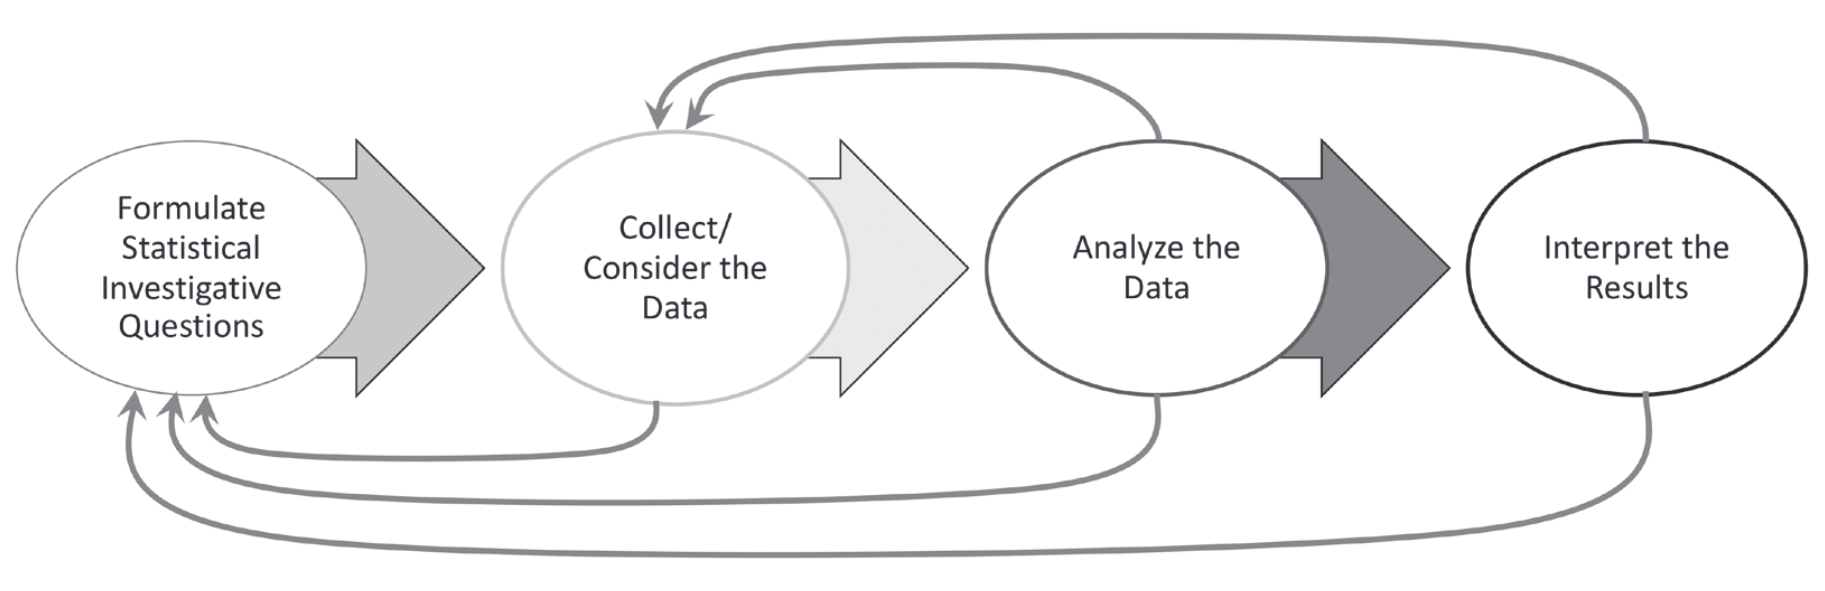
\includegraphics[width=\textwidth]{figs/050-intro/gaise2-stat_problem_solving_process.png}
        \caption[GAISE II Pre-K-12 Statistical Problem-Solving Process]{
        Reproduction of the GAISE II Pre-K-12 statistical problem-solving process \cite{gaise2k12}.
        }
        \label{fig:gaisek-12}
    \end{figure}

    The emphasis around incorporating non-traditional data sources
    (e.g., GPS coordinates from a fitness application)
    for analysis and interpretation
    hopes to give younger learners an earlier explore to the data science process
    \cite{gaise2k12}.

\end{document}
